\documentclass[12pt,landscape]{article}

%\usepackage{lmodern}
\usepackage{amssymb,amsmath}
\usepackage{bm}
\usepackage{graphicx}
\usepackage{microtype}
\usepackage{hyperref}
\usepackage{bigints}
\pagestyle{empty}
\usepackage{titlesec}
\titleformat*{\section}{\LARGE\bfseries}
\titleformat*{\subsection}{\LARGE\bfseries}
\titleformat*{\subsubsection}{\LARGE\bfseries}
\setlength{\parindent}{0pt}
\setlength{\parskip}{1.2ex}
\setlength{\parindent}{0pt}
\setlength{\parskip}{1.2ex}

\setlength{\oddsidemargin}{-16mm}
\setlength{\textwidth}{260mm}
\setlength{\columnsep}{0.5in}
\setlength{\columnseprule}{1pt}
\setlength{\textheight}{202mm}
\setlength{\topmargin}{-32mm}
\setlength{\headsep}{0.25in}

\hypersetup
       {   pdfauthor = { Marco Fasondini },
           pdftitle={ foo },
           colorlinks=TRUE,
           linkcolor=black,
           citecolor=blue,
           urlcolor=blue
       }




\usepackage{upquote}
\usepackage{listings}
\usepackage{xcolor}
\lstset{
    basicstyle=\ttfamily\footnotesize,
    upquote=true,
    breaklines=true,
    breakindent=0pt,
    keepspaces=true,
    showspaces=false,
    columns=fullflexible,
    showtabs=false,
    showstringspaces=false,
    escapeinside={(*@}{@*)},
    extendedchars=true,
}
\newcommand{\HLJLt}[1]{#1}
\newcommand{\HLJLw}[1]{#1}
\newcommand{\HLJLe}[1]{#1}
\newcommand{\HLJLeB}[1]{#1}
\newcommand{\HLJLo}[1]{#1}
\newcommand{\HLJLk}[1]{\textcolor[RGB]{148,91,176}{\textbf{#1}}}
\newcommand{\HLJLkc}[1]{\textcolor[RGB]{59,151,46}{\textit{#1}}}
\newcommand{\HLJLkd}[1]{\textcolor[RGB]{214,102,97}{\textit{#1}}}
\newcommand{\HLJLkn}[1]{\textcolor[RGB]{148,91,176}{\textbf{#1}}}
\newcommand{\HLJLkp}[1]{\textcolor[RGB]{148,91,176}{\textbf{#1}}}
\newcommand{\HLJLkr}[1]{\textcolor[RGB]{148,91,176}{\textbf{#1}}}
\newcommand{\HLJLkt}[1]{\textcolor[RGB]{148,91,176}{\textbf{#1}}}
\newcommand{\HLJLn}[1]{#1}
\newcommand{\HLJLna}[1]{#1}
\newcommand{\HLJLnb}[1]{#1}
\newcommand{\HLJLnbp}[1]{#1}
\newcommand{\HLJLnc}[1]{#1}
\newcommand{\HLJLncB}[1]{#1}
\newcommand{\HLJLnd}[1]{\textcolor[RGB]{214,102,97}{#1}}
\newcommand{\HLJLne}[1]{#1}
\newcommand{\HLJLneB}[1]{#1}
\newcommand{\HLJLnf}[1]{\textcolor[RGB]{66,102,213}{#1}}
\newcommand{\HLJLnfm}[1]{\textcolor[RGB]{66,102,213}{#1}}
\newcommand{\HLJLnp}[1]{#1}
\newcommand{\HLJLnl}[1]{#1}
\newcommand{\HLJLnn}[1]{#1}
\newcommand{\HLJLno}[1]{#1}
\newcommand{\HLJLnt}[1]{#1}
\newcommand{\HLJLnv}[1]{#1}
\newcommand{\HLJLnvc}[1]{#1}
\newcommand{\HLJLnvg}[1]{#1}
\newcommand{\HLJLnvi}[1]{#1}
\newcommand{\HLJLnvm}[1]{#1}
\newcommand{\HLJLl}[1]{#1}
\newcommand{\HLJLld}[1]{\textcolor[RGB]{148,91,176}{\textit{#1}}}
\newcommand{\HLJLs}[1]{\textcolor[RGB]{201,61,57}{#1}}
\newcommand{\HLJLsa}[1]{\textcolor[RGB]{201,61,57}{#1}}
\newcommand{\HLJLsb}[1]{\textcolor[RGB]{201,61,57}{#1}}
\newcommand{\HLJLsc}[1]{\textcolor[RGB]{201,61,57}{#1}}
\newcommand{\HLJLsd}[1]{\textcolor[RGB]{201,61,57}{#1}}
\newcommand{\HLJLsdB}[1]{\textcolor[RGB]{201,61,57}{#1}}
\newcommand{\HLJLsdC}[1]{\textcolor[RGB]{201,61,57}{#1}}
\newcommand{\HLJLse}[1]{\textcolor[RGB]{59,151,46}{#1}}
\newcommand{\HLJLsh}[1]{\textcolor[RGB]{201,61,57}{#1}}
\newcommand{\HLJLsi}[1]{#1}
\newcommand{\HLJLso}[1]{\textcolor[RGB]{201,61,57}{#1}}
\newcommand{\HLJLsr}[1]{\textcolor[RGB]{201,61,57}{#1}}
\newcommand{\HLJLss}[1]{\textcolor[RGB]{201,61,57}{#1}}
\newcommand{\HLJLssB}[1]{\textcolor[RGB]{201,61,57}{#1}}
\newcommand{\HLJLnB}[1]{\textcolor[RGB]{59,151,46}{#1}}
\newcommand{\HLJLnbB}[1]{\textcolor[RGB]{59,151,46}{#1}}
\newcommand{\HLJLnfB}[1]{\textcolor[RGB]{59,151,46}{#1}}
\newcommand{\HLJLnh}[1]{\textcolor[RGB]{59,151,46}{#1}}
\newcommand{\HLJLni}[1]{\textcolor[RGB]{59,151,46}{#1}}
\newcommand{\HLJLnil}[1]{\textcolor[RGB]{59,151,46}{#1}}
\newcommand{\HLJLnoB}[1]{\textcolor[RGB]{59,151,46}{#1}}
\newcommand{\HLJLoB}[1]{\textcolor[RGB]{102,102,102}{\textbf{#1}}}
\newcommand{\HLJLow}[1]{\textcolor[RGB]{102,102,102}{\textbf{#1}}}
\newcommand{\HLJLp}[1]{#1}
\newcommand{\HLJLc}[1]{\textcolor[RGB]{153,153,119}{\textit{#1}}}
\newcommand{\HLJLch}[1]{\textcolor[RGB]{153,153,119}{\textit{#1}}}
\newcommand{\HLJLcm}[1]{\textcolor[RGB]{153,153,119}{\textit{#1}}}
\newcommand{\HLJLcp}[1]{\textcolor[RGB]{153,153,119}{\textit{#1}}}
\newcommand{\HLJLcpB}[1]{\textcolor[RGB]{153,153,119}{\textit{#1}}}
\newcommand{\HLJLcs}[1]{\textcolor[RGB]{153,153,119}{\textit{#1}}}
\newcommand{\HLJLcsB}[1]{\textcolor[RGB]{153,153,119}{\textit{#1}}}
\newcommand{\HLJLg}[1]{#1}
\newcommand{\HLJLgd}[1]{#1}
\newcommand{\HLJLge}[1]{#1}
\newcommand{\HLJLgeB}[1]{#1}
\newcommand{\HLJLgh}[1]{#1}
\newcommand{\HLJLgi}[1]{#1}
\newcommand{\HLJLgo}[1]{#1}
\newcommand{\HLJLgp}[1]{#1}
\newcommand{\HLJLgs}[1]{#1}
\newcommand{\HLJLgsB}[1]{#1}
\newcommand{\HLJLgt}[1]{#1}



\def\qqand{\qquad\hbox{and}\qquad}
\def\qqfor{\qquad\hbox{for}\qquad}
\def\qqas{\qquad\hbox{as}\qquad}
\def\half{ {1 \over 2} }
\def\D{ {\rm d} }
\def\I{ {\rm i} }
\def\E{ {\rm e} }
\def\C{ {\mathbb C} }
\def\R{ {\mathbb R} }
\def\H{ {\mathbb H} }
\def\Z{ {\mathbb Z} }
\def\CC{ {\cal C} }
\def\FF{ {\cal F} }
\def\HH{ {\cal H} }
\def\LL{ {\cal L} }
\def\vc#1{ {\mathbf #1} }
\def\bbC{ {\mathbb C} }



\def\fR{ f_{\rm R} }
\def\fL{ f_{\rm L} }

\def\qqqquad{\qquad\qquad}
\def\qqwhere{\qquad\hbox{where}\qquad}
\def\Res_#1{\underset{#1}{\rm Res}\,}
\def\sech{ {\rm sech}\, }
\def\acos{ {\rm acos}\, }
\def\asin{ {\rm asin}\, }
\def\atan{ {\rm atan}\, }
\def\Ei{ {\rm Ei}\, }
\def\upepsilon{\varepsilon}


\def\Xint#1{ \mathchoice
   {\XXint\displaystyle\textstyle{#1} }%
   {\XXint\textstyle\scriptstyle{#1} }%
   {\XXint\scriptstyle\scriptscriptstyle{#1} }%
   {\XXint\scriptscriptstyle\scriptscriptstyle{#1} }%
   \!\int}
\def\XXint#1#2#3{ {\setbox0=\hbox{$#1{#2#3}{\int}$}
     \vcenter{\hbox{$#2#3$}}\kern-.5\wd0} }
\def\ddashint{\Xint=}
\def\dashint{\Xint-}
% \def\dashint
\def\infdashint{\dashint_{-\infty}^\infty}




\def\addtab#1={#1\;&=}
\def\ccr{\\\addtab}
\def\ip<#1>{\left\langle{#1}\right\rangle}
\def\dx{\D x}
\def\dt{\D t}
\def\dz{\D z}
\def\ds{\D s}

\def\rR{ {\rm R} }
\def\rL{ {\rm L} }

\def\norm#1{\left\| #1 \right\|}

\def\pr(#1){\left({#1}\right)}
\def\br[#1]{\left[{#1}\right]}

\def\abs#1{\left|{#1}\right|}
\def\fpr(#1){\!\pr({#1})}

\def\sopmatrix#1{ \begin{pmatrix}#1\end{pmatrix} }

\def\endash{–}
\def\emdash{—}
\def\mdblksquare{\blacksquare}
\def\lgblksquare{\blacksquare}
\def\scre{\E}
\def\mapengine#1,#2.{\mapfunction{#1}\ifx\void#2\else\mapengine #2.\fi }

\def\map[#1]{\mapengine #1,\void.}

\def\mapenginesep_#1#2,#3.{\mapfunction{#2}\ifx\void#3\else#1\mapengine #3.\fi }

\def\mapsep_#1[#2]{\mapenginesep_{#1}#2,\void.}


\def\vcbr[#1]{\pr(#1)}


\def\bvect[#1,#2]{
{
\def\dots{\cdots}
\def\mapfunction##1{\ | \  ##1}
	\sopmatrix{
		 \,#1\map[#2]\,
	}
}
}



\def\vect[#1]{
{\def\dots{\ldots}
	\vcbr[{#1}]
} }

\def\vectt[#1]{
{\def\dots{\ldots}
	\vect[{#1}]^{\top}
} }

\def\Vectt[#1]{
{
\def\mapfunction##1{##1 \cr}
\def\dots{\vdots}
	\begin{pmatrix}
		\map[#1]
	\end{pmatrix}
} }

\def\addtab#1={#1\;&=}
\def\ccr{\\\addtab}

\def\questionequals{= \!\!\!\!\!\!{\scriptstyle ? \atop }\,\,\,}

\def\cent#1{\begin{center}#1\end{center} }

\lstset{
    basicstyle=\ttfamily,
	}

\begin{document}
{\LARGE
\sf
\textbf{Applied Complex Analysis (2021)}

\section{Lecture 2: Cauchy's integral formula and Taylor series}
\subsection{Holomorphicity, Cauchy's theorem, and Analyticity}
A beautiful feature of complex analysis is one starts with a very weak assumption of holomorphicity, essentially complex-differentiability in an open set, deduce Cauchy's theorem and Cauchy's integral formula, which then imply analyticity. That is, if we assume a function is one-time complex differentiable, then it has an infinite number of derivatives.

These results are built up as follows:

\begin{itemize}
\item[1. ] Holomorphic functions


\item[2. ] Cauchy's theorem


\item[3. ] Deformation of contours


\item[4. ] Cauchy's integral formula


\item[5. ] Analyticity and Taylor series

\end{itemize}
\newpage
\subsubsection{Holomorphic functions}
\textbf{Definition (Complex-differentiability)} Let $D \subset {\mathbb C}$ be an open set.  A function $f : D \rightarrow {\mathbb C}$ is called \emph{complex-differentiable} at a point $z_0 \in D$ if

\[
   f'(z_0) =  \lim_{z \rightarrow z_0} {f(z) - f(z_0) \over z - z_0}
\]
exists, for any angle of approach to $z_0$.

\textbf{Definition (Holomorphic)} Let $D \subset {\mathbb C}$ be an open set.  A function $f : D \rightarrow {\mathbb C}$ is called \emph{holomorphic} in $D$ if it is complex-differentiable at all $z \in D$.

\textbf{Definition (Entire)} A function is \emph{entire} if it is holomorphic in ${\mathbb C}$

\newpage
\emph{Examples}

\begin{itemize}
\item[1. ] \[
1
\]
is entire


\item[2. ] \[
z
\]
is entire


\item[3. ] \[
1/z
\]
is holomorphic in ${\mathbb C} \backslash \{0\}$


\item[4. ] \[
\sin z
\]
is entire


\item[5. ] \[
\csc z
\]
is holomorphic in ${\mathbb C} \backslash \{\ldots,-2\pi,-\pi,0,\pi,2\pi,\ldots\}$


\item[6. ] \[
\sqrt z
\]
is holomorphic in ${\mathbb C} \backslash (-\infty,0]$

\end{itemize}
\subsubsection{Cauchy's theorem}
\textbf{Definition (Contour)} A \emph{contour}  is a continuous \& piecewise-continuously differentiable function $\gamma : [a,b] \rightarrow {\mathbb C}$.

\textbf{Definition (Simple)} A \emph{simple contour} is a contour that is 1-to-1, except possibly at the endpoints $a$ and $b$.

\textbf{Definition (Closed)} A \emph{closed contour} is a contour such that $\gamma(a) = \gamma(b)$

\emph{Examples of contours}

\begin{itemize}
\item[1. ] A line segment $t \in [a,b]$ is a simple contour, with $\gamma(t) =  t$


\item[2. ] An arc from $re^{ia}$ to $re^{ib}$ with $-\pi < a < b < \pi$ is a simple contour, with $\gamma(t) =  re^{i t}$


\item[3. ] A Circle of radius $r$ is a closed simple contour, with $\gamma(t) = re^{i t}$ and $a = -\pi$, $b = \pi$


\item[4. ] \[
\gamma(t) = \cos (t+i)^2
\]
for $[a,b] = [-2\pi/3,2\pi/3]$ defines a contour that is neither simple nor closed

\end{itemize}
\newpage
\begin{lstlisting}
(*@\HLJLk{using}@*) (*@\HLJLn{Plots}@*)(*@\HLJLp{,}@*) (*@\HLJLn{ComplexPhasePortrait}@*)(*@\HLJLp{,}@*) (*@\HLJLn{SpecialFunctions}@*)(*@\HLJLp{,}@*) (*@\HLJLn{ApproxFun}@*)
(*@\HLJLn{a}@*)(*@\HLJLp{,}@*)(*@\HLJLn{b}@*) (*@\HLJLoB{=}@*) (*@\HLJLoB{-}@*)(*@\HLJLni{2}@*)(*@\HLJLn{\ensuremath{\pi}}@*)(*@\HLJLoB{/}@*)(*@\HLJLni{3}@*)(*@\HLJLp{,}@*) (*@\HLJLni{2}@*)(*@\HLJLn{\ensuremath{\pi}}@*)(*@\HLJLoB{/}@*)(*@\HLJLni{3}@*)
(*@\HLJLn{tt}@*) (*@\HLJLoB{=}@*) (*@\HLJLnf{range}@*)(*@\HLJLp{(}@*)(*@\HLJLn{a}@*)(*@\HLJLp{,}@*) (*@\HLJLn{stop}@*)(*@\HLJLoB{=}@*)(*@\HLJLn{b}@*)(*@\HLJLp{,}@*) (*@\HLJLn{length}@*)(*@\HLJLoB{=}@*)(*@\HLJLni{1000}@*)(*@\HLJLp{)}@*)

(*@\HLJLn{\ensuremath{\gamma}}@*) (*@\HLJLoB{=}@*) (*@\HLJLn{t}@*) (*@\HLJLoB{->}@*) (*@\HLJLnf{cos}@*)(*@\HLJLp{((}@*)(*@\HLJLn{t}@*)(*@\HLJLoB{+}@*)(*@\HLJLn{im}@*)(*@\HLJLp{)}@*)(*@\HLJLoB{{\textasciicircum}}@*)(*@\HLJLni{2}@*)(*@\HLJLp{)}@*)

(*@\HLJLnf{plot}@*)(*@\HLJLp{(}@*)(*@\HLJLn{real}@*)(*@\HLJLoB{.}@*)(*@\HLJLp{(}@*)(*@\HLJLn{\ensuremath{\gamma}}@*)(*@\HLJLoB{.}@*)(*@\HLJLp{(}@*)(*@\HLJLn{tt}@*)(*@\HLJLp{)),}@*) (*@\HLJLn{imag}@*)(*@\HLJLoB{.}@*)(*@\HLJLp{(}@*)(*@\HLJLn{\ensuremath{\gamma}}@*)(*@\HLJLoB{.}@*)(*@\HLJLp{(}@*)(*@\HLJLn{tt}@*)(*@\HLJLp{));}@*) (*@\HLJLn{ratio}@*)(*@\HLJLoB{=}@*)(*@\HLJLnfB{1.0}@*)(*@\HLJLp{,}@*) (*@\HLJLn{legend}@*)(*@\HLJLoB{=}@*)(*@\HLJLkc{false}@*)(*@\HLJLp{,}@*) (*@\HLJLn{arrow}@*)(*@\HLJLoB{=}@*)(*@\HLJLkc{true}@*)(*@\HLJLp{)}@*)
\end{lstlisting}

\cent{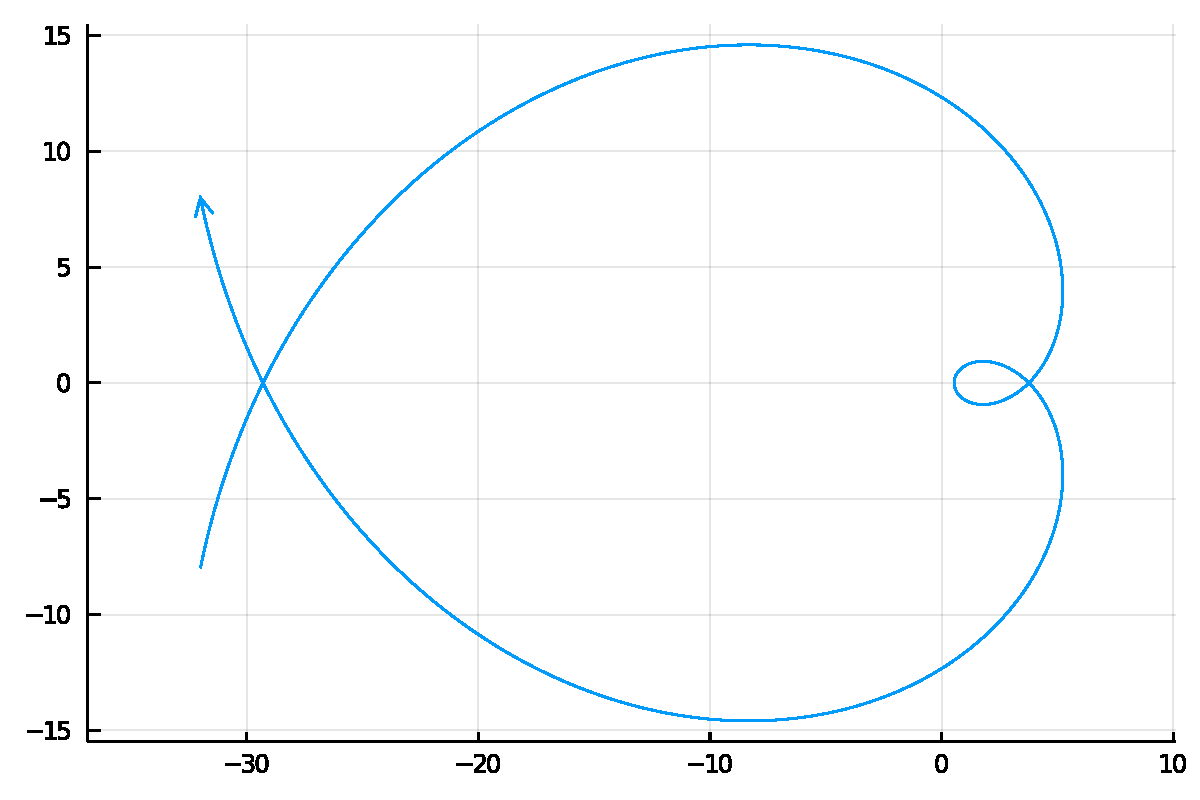
\includegraphics[width=0.7\linewidth]{C:/Users/mfaso/OneDrive/Documents/GitHub/M3M6AppliedComplexAnalysis/output/figures/Lecture2_1_1.pdf}}
\newpage
\begin{itemize}
\item[5. ] \[
\gamma(t) = e^{i t} + e^{2i t}
\]
for $[a,b] = [-\pi,\pi]$ defines a contour that is closed but not simple

\end{itemize}

\begin{lstlisting}
(*@\HLJLn{a}@*)(*@\HLJLp{,}@*)(*@\HLJLn{b}@*) (*@\HLJLoB{=}@*) (*@\HLJLoB{-}@*)(*@\HLJLn{\ensuremath{\pi}}@*)(*@\HLJLp{,}@*) (*@\HLJLn{\ensuremath{\pi}}@*)
(*@\HLJLn{tt}@*) (*@\HLJLoB{=}@*) (*@\HLJLnf{range}@*)(*@\HLJLp{(}@*)(*@\HLJLn{a}@*)(*@\HLJLp{,}@*) (*@\HLJLn{stop}@*)(*@\HLJLoB{=}@*)(*@\HLJLn{b}@*)(*@\HLJLp{,}@*) (*@\HLJLn{length}@*)(*@\HLJLoB{=}@*)(*@\HLJLni{1000}@*)(*@\HLJLp{)}@*)

(*@\HLJLn{\ensuremath{\gamma}}@*) (*@\HLJLoB{=}@*) (*@\HLJLn{t}@*) (*@\HLJLoB{->}@*) (*@\HLJLnf{exp}@*)(*@\HLJLp{(}@*)(*@\HLJLn{im}@*)(*@\HLJLoB{*}@*)(*@\HLJLn{t}@*)(*@\HLJLp{)}@*) (*@\HLJLoB{+}@*)(*@\HLJLnf{exp}@*)(*@\HLJLp{(}@*)(*@\HLJLni{2}@*)(*@\HLJLn{im}@*)(*@\HLJLoB{*}@*)(*@\HLJLn{t}@*)(*@\HLJLp{)}@*)

(*@\HLJLnf{plot}@*)(*@\HLJLp{(}@*)(*@\HLJLn{real}@*)(*@\HLJLoB{.}@*)(*@\HLJLp{(}@*)(*@\HLJLn{\ensuremath{\gamma}}@*)(*@\HLJLoB{.}@*)(*@\HLJLp{(}@*)(*@\HLJLn{tt}@*)(*@\HLJLp{)),}@*) (*@\HLJLn{imag}@*)(*@\HLJLoB{.}@*)(*@\HLJLp{(}@*)(*@\HLJLn{\ensuremath{\gamma}}@*)(*@\HLJLoB{.}@*)(*@\HLJLp{(}@*)(*@\HLJLn{tt}@*)(*@\HLJLp{));}@*) (*@\HLJLn{ratio}@*)(*@\HLJLoB{=}@*)(*@\HLJLnfB{1.0}@*)(*@\HLJLp{,}@*) (*@\HLJLn{legend}@*)(*@\HLJLoB{=}@*)(*@\HLJLkc{false}@*)(*@\HLJLp{,}@*) (*@\HLJLn{arrow}@*)(*@\HLJLoB{=}@*)(*@\HLJLkc{true}@*)(*@\HLJLp{)}@*)
\end{lstlisting}

\cent{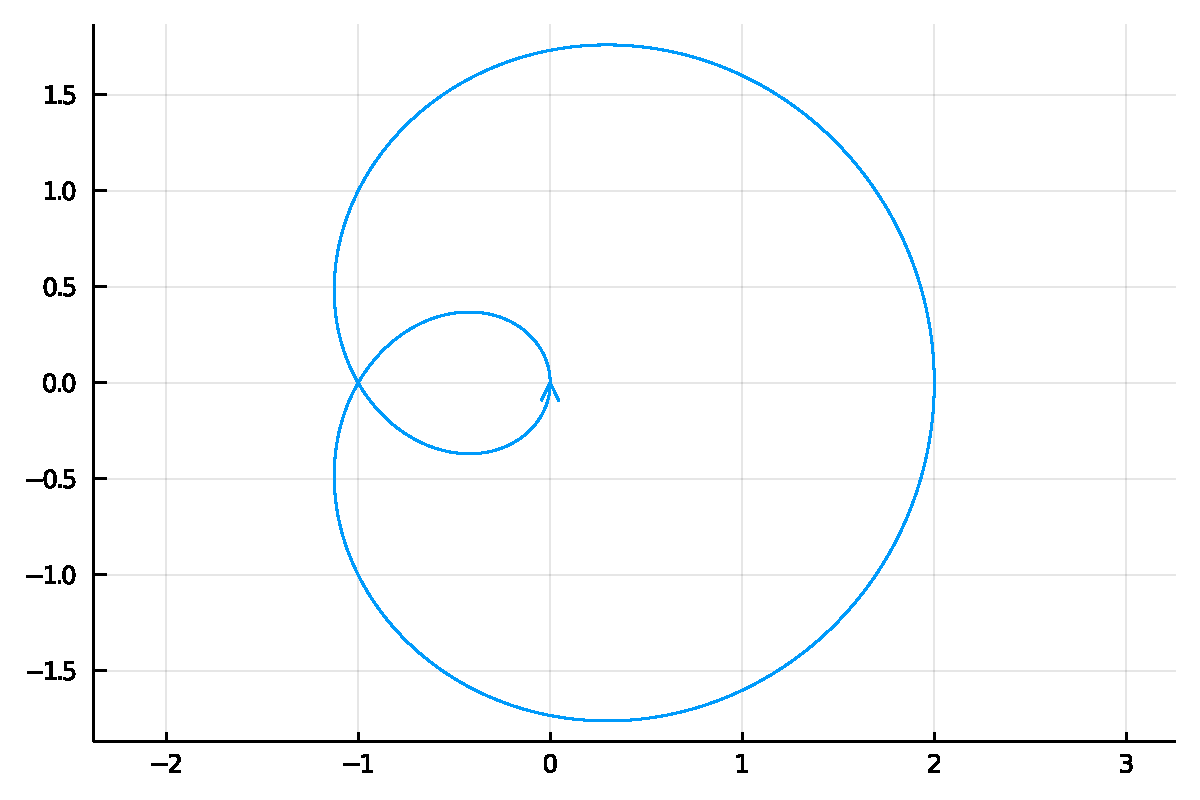
\includegraphics[width=0.6\linewidth]{C:/Users/mfaso/OneDrive/Documents/GitHub/M3M6AppliedComplexAnalysis/output/figures/Lecture2_2_1.pdf}}

\textbf{Definition (Contour integral)} The \emph{contour integral} over $\gamma$ is defined by

\[
\int_\gamma f(z) dz := \int_a^b f(\gamma(t)) \gamma'(t) dt
\]
An important property of a contour is its \emph{arclength}:

\textbf{Definition (Arclength)} The \emph{arclength} of $\gamma$ is defined as

\[
    {\cal L}(\gamma) := \int_a^b |\gamma'(t)| dt
\]
A very useful result is that we can use the maximum and arclength to bound integrals:

\textbf{Proposition (ML)} Let $f : \gamma \rightarrow {\mathbb C}$ and

\[
        M = \sup_{z \in \gamma} |f(z)|
\]
Then

\[
\left|\int_\gamma f(z) dz \right| \leq M {\cal L}(\gamma)
\]
\textbf{Proposition} If $f(z)$ is holomorphic on $\gamma$, then $\displaystyle{\int_\gamma f'(z) dz = f(\gamma(b)) - f(\gamma(a))}$

\textbf{Theorem (Cauchy)} If $f$ is holomorphic inside and on a closed contour $\gamma$, then 
\begin{align*}
\oint f(z) dz = 0
\end{align*}
%\[
%\oint_\gamma f(z) dz = 0
%\]
\subsubsection{Deformation of contours}
\textbf{Definition (Domain)} A \emph{domain} is a non-empty, open and connected set $D \subset {\mathbb C}$.

\textbf{Definition (Homotopic)} Two closed contours $\gamma_1 : [a,b] \rightarrow D$ and $\gamma_2 \rightarrow D$ in a domain $D$ are \emph{homotopic} if they can be continuously deformed to one-another while remaining in $D$.

\textbf{Theorem (Deformation of contours)} Let $f(z)$ be holomorphic in a domain $D$. Let $\gamma_1$ and $\gamma_2$ be two closed homotopic contours. Then

\[
    \int_{\gamma_1} f(z) dz = \int_{\gamma_2} f(z) dz
\]
\textbf{Definition (Simply connected)} A domain is \emph{simply connected} if every closed contour is homotopic to a point in the domain.

\textbf{Corollary (Deformation of contours on simply connected domains)} Let $f(z)$ be holomorphic in a simply-connected domain $D$. If $\gamma_1$ and $\gamma_2$ are two contours in $D$ with the same endpoints, then

\[
    \int_{\gamma_1} f(z) dz = \int_{\gamma_2} f(z) dz
\]
\newpage
\subsubsection{Demonstration}
We can usually infer the domain where a function is holomorphic from a phase portrait, here we see that ${\rm arcsinh}\, z$ has cuts on $[\I,\I \infty)$ and $[-\I,-\I \infty)$, and a zero  (red-green-blue-red) at zero, hence we can infer that it is holomorphic in $\C \backslash ([\I,\I \infty) \cup [-\I,-\I \infty))$.


\begin{lstlisting}
(*@\HLJLnf{phaseplot}@*)(*@\HLJLp{(}@*)(*@\HLJLoB{-}@*)(*@\HLJLnfB{4..4}@*)(*@\HLJLp{,}@*) (*@\HLJLoB{-}@*)(*@\HLJLnfB{4..4}@*)(*@\HLJLp{,}@*) (*@\HLJLn{z}@*) (*@\HLJLoB{->}@*) (*@\HLJLnf{asinh}@*)(*@\HLJLp{(}@*)(*@\HLJLn{z}@*)(*@\HLJLp{))}@*)
\end{lstlisting}

\cent{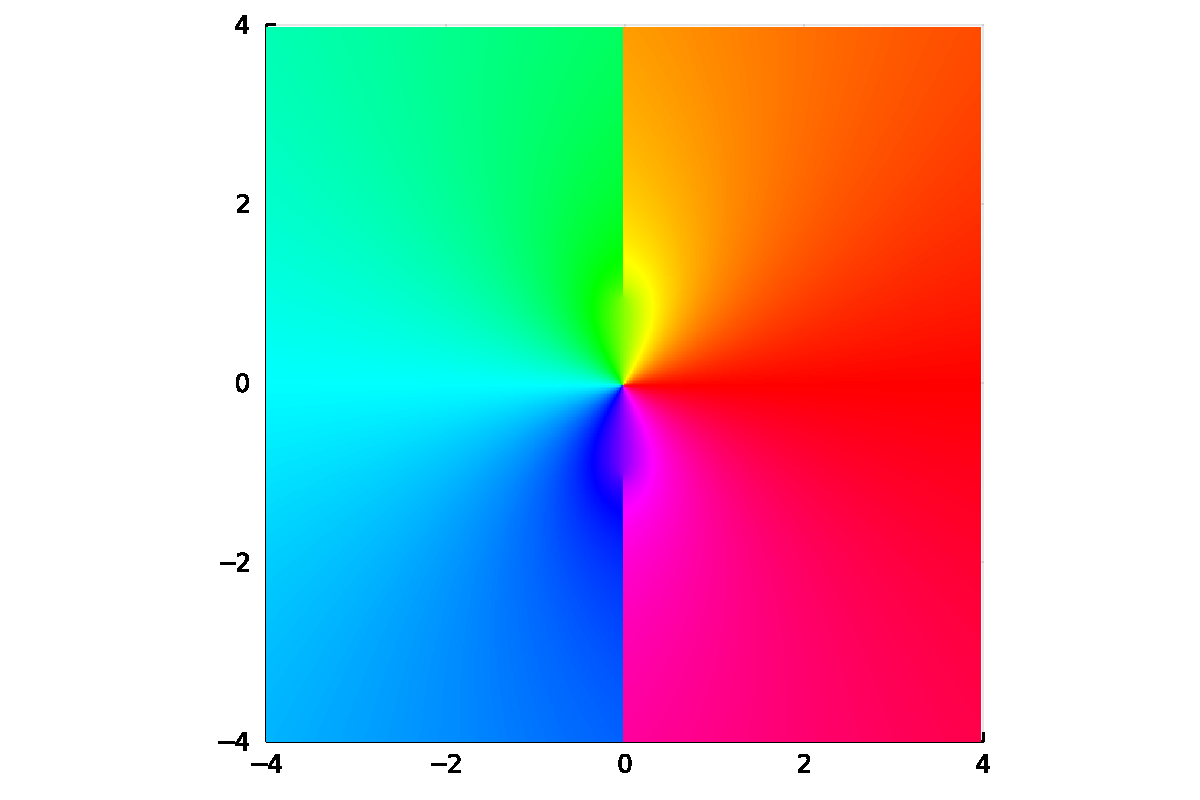
\includegraphics[width=0.8\linewidth]{C:/Users/mfaso/OneDrive/Documents/GitHub/M3M6AppliedComplexAnalysis/output/figures/Lecture2_3_1.pdf}}

The following example $\sqrt{z-1} \sqrt{z+1}$ is analytic in ${\mathbb C}\backslash [-1,1]$ and will be returned to:


\begin{lstlisting}
(*@\HLJLnf{phaseplot}@*)(*@\HLJLp{(}@*)(*@\HLJLoB{-}@*)(*@\HLJLnfB{4..4}@*)(*@\HLJLp{,}@*) (*@\HLJLoB{-}@*)(*@\HLJLnfB{4..4}@*)(*@\HLJLp{,}@*) (*@\HLJLn{z}@*) (*@\HLJLoB{->}@*) (*@\HLJLnf{sqrt}@*)(*@\HLJLp{(}@*)(*@\HLJLn{z}@*)(*@\HLJLoB{-}@*)(*@\HLJLni{1}@*)(*@\HLJLp{)}@*)(*@\HLJLnf{sqrt}@*)(*@\HLJLp{(}@*)(*@\HLJLn{z}@*)(*@\HLJLoB{+}@*)(*@\HLJLni{1}@*)(*@\HLJLp{))}@*)
\end{lstlisting}

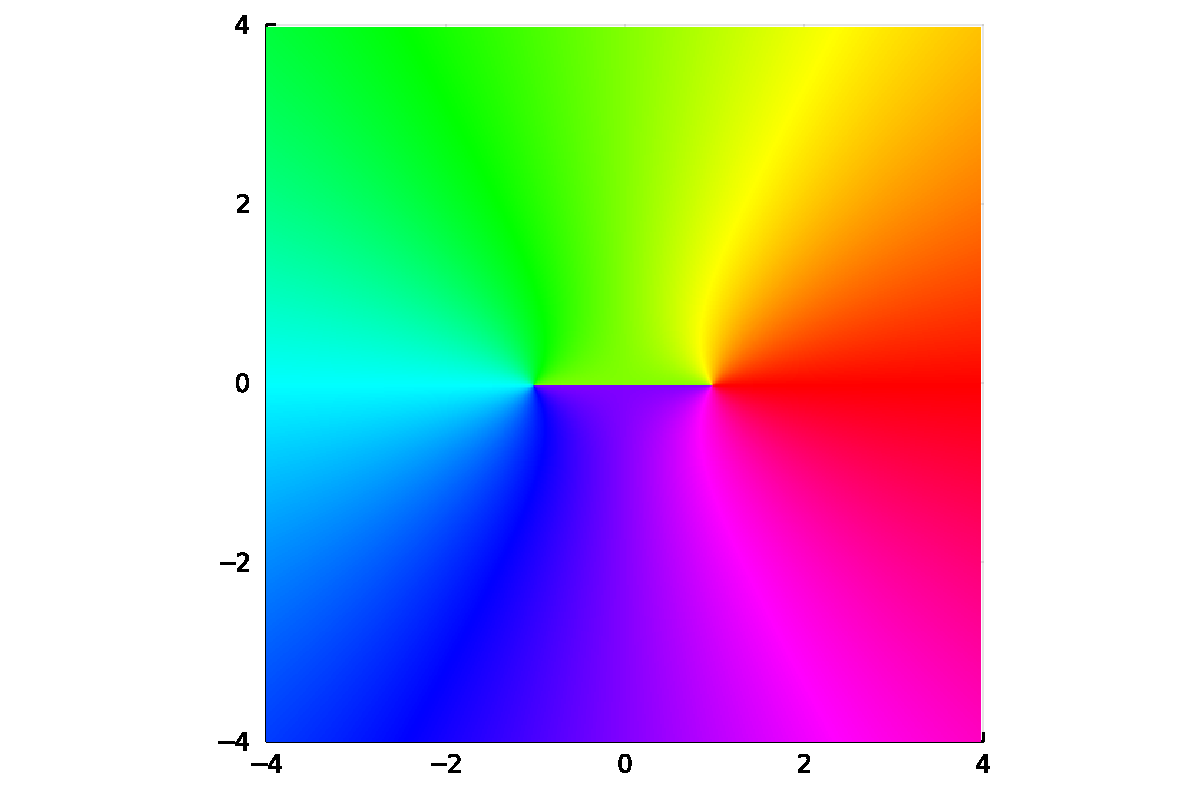
\includegraphics[width=\linewidth]{C:/Users/mfaso/OneDrive/Documents/GitHub/M3M6AppliedComplexAnalysis/output/figures/Lecture2_4_1.pdf}

The notion of integration over a contour in the complex plane is independent of the notion of holomorphicity. For example, we can happily define the integral for non-holomorphic functions such as $\Re \E^z = \E^x \cos y$:


\begin{lstlisting}
(*@\HLJLn{f}@*) (*@\HLJLoB{=}@*) (*@\HLJLnf{Fun}@*)(*@\HLJLp{(}@*) (*@\HLJLn{z}@*) (*@\HLJLoB{->}@*) (*@\HLJLnf{real}@*)(*@\HLJLp{(}@*)(*@\HLJLnf{exp}@*)(*@\HLJLp{(}@*)(*@\HLJLn{z}@*)(*@\HLJLp{)),}@*) (*@\HLJLnf{Arc}@*)(*@\HLJLp{(}@*)(*@\HLJLnfB{0.}@*)(*@\HLJLp{,}@*)(*@\HLJLnfB{1.}@*)(*@\HLJLp{,(}@*)(*@\HLJLni{0}@*)(*@\HLJLp{,}@*)(*@\HLJLn{\ensuremath{\pi}}@*)(*@\HLJLoB{/}@*)(*@\HLJLni{2}@*)(*@\HLJLp{)))}@*)  (*@\HLJLcs{{\#}}@*) (*@\HLJLcs{Not}@*) (*@\HLJLcs{holomorphic!}@*)

(*@\HLJLnf{plot}@*)(*@\HLJLp{(}@*)(*@\HLJLnf{domain}@*)(*@\HLJLp{(}@*)(*@\HLJLn{f}@*)(*@\HLJLp{);}@*) (*@\HLJLn{legend}@*)(*@\HLJLoB{=}@*)(*@\HLJLkc{false}@*)(*@\HLJLp{,}@*) (*@\HLJLn{ratio}@*)(*@\HLJLoB{=}@*)(*@\HLJLnfB{1.0}@*)(*@\HLJLp{,}@*) (*@\HLJLn{arrow}@*)(*@\HLJLoB{=}@*)(*@\HLJLkc{true}@*)(*@\HLJLp{)}@*)
\end{lstlisting}

\cent{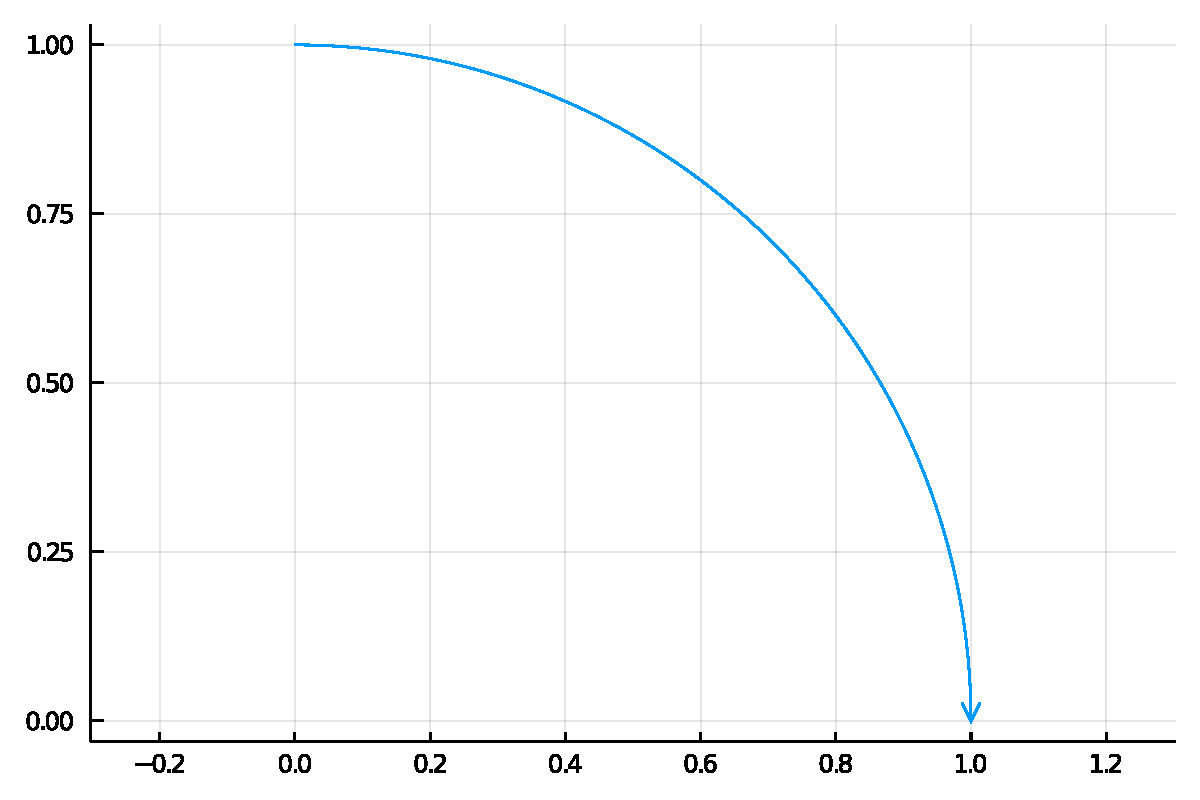
\includegraphics[width=0.8\linewidth]{C:/Users/mfaso/OneDrive/Documents/GitHub/M3M6AppliedComplexAnalysis/output/figures/Lecture2_5_1.pdf}}

\begin{lstlisting}
(*@\HLJLnf{sum}@*)(*@\HLJLp{(}@*)(*@\HLJLn{f}@*)(*@\HLJLp{)}@*)  (*@\HLJLcs{{\#}}@*) (*@\HLJLcs{this}@*) (*@\HLJLcs{means}@*) (*@\HLJLcs{contour}@*) (*@\HLJLcs{integral}@*)
\end{lstlisting}

\begin{lstlisting}
-1.2485382363935422 + 1.949326343919058im
\end{lstlisting}


This is defined in terms of a parameterization, and so the following real integral gives the same result:


\begin{lstlisting}
(*@\HLJLn{g}@*) (*@\HLJLoB{=}@*) (*@\HLJLn{im}@*)(*@\HLJLoB{*}@*)(*@\HLJLnf{Fun}@*)(*@\HLJLp{(}@*)(*@\HLJLn{t}@*)(*@\HLJLoB{->}@*) (*@\HLJLnf{f}@*)(*@\HLJLp{(}@*)(*@\HLJLnf{exp}@*)(*@\HLJLp{(}@*)(*@\HLJLn{im}@*)(*@\HLJLoB{*}@*)(*@\HLJLn{t}@*)(*@\HLJLp{))}@*)(*@\HLJLoB{*}@*)(*@\HLJLnf{exp}@*)(*@\HLJLp{(}@*)(*@\HLJLn{im}@*)(*@\HLJLoB{*}@*)(*@\HLJLn{t}@*)(*@\HLJLp{),}@*) (*@\HLJLni{0}@*) (*@\HLJLoB{..}@*) (*@\HLJLn{\ensuremath{\pi}}@*)(*@\HLJLoB{/}@*)(*@\HLJLni{2}@*)(*@\HLJLp{)}@*)
(*@\HLJLnf{sum}@*)(*@\HLJLp{(}@*) (*@\HLJLn{g}@*) (*@\HLJLp{)}@*)  (*@\HLJLcs{{\#}}@*) (*@\HLJLcs{this}@*) (*@\HLJLcs{is}@*) (*@\HLJLcs{standard}@*) (*@\HLJLcs{integral}@*)
\end{lstlisting}

\begin{lstlisting}
-1.248538236393543 + 1.9493263439190578im
\end{lstlisting}


The following show that the contour of integration does not affect the integral for holomorphic functions:


\begin{lstlisting}
(*@\HLJLn{f}@*) (*@\HLJLoB{=}@*) (*@\HLJLnf{Fun}@*)(*@\HLJLp{(}@*) (*@\HLJLn{z}@*) (*@\HLJLoB{->}@*) (*@\HLJLnf{exp}@*)(*@\HLJLp{(}@*)(*@\HLJLn{z}@*)(*@\HLJLp{),}@*) (*@\HLJLnf{Arc}@*)(*@\HLJLp{(}@*)(*@\HLJLnfB{0.}@*)(*@\HLJLp{,}@*)(*@\HLJLnfB{1.}@*)(*@\HLJLp{,(}@*)(*@\HLJLni{0}@*)(*@\HLJLp{,}@*)(*@\HLJLn{\ensuremath{\pi}}@*)(*@\HLJLoB{/}@*)(*@\HLJLni{2}@*)(*@\HLJLp{)))}@*) (*@\HLJLcs{{\#}integrate}@*) (*@\HLJLcs{over}@*) (*@\HLJLcs{an}@*) (*@\HLJLcs{arc}@*)
(*@\HLJLnf{sum}@*)(*@\HLJLp{(}@*)(*@\HLJLn{f}@*)(*@\HLJLp{)}@*)  (*@\HLJLp{,}@*) (*@\HLJLnf{f}@*)(*@\HLJLp{(}@*)(*@\HLJLn{im}@*)(*@\HLJLp{)}@*)(*@\HLJLoB{-}@*)(*@\HLJLnf{f}@*)(*@\HLJLp{(}@*)(*@\HLJLni{1}@*)(*@\HLJLp{)}@*)
\end{lstlisting}

\begin{lstlisting}
(-2.1779795225909053 + 0.8414709848078971im, -2.177979522590906 + 0.8414709
848078968im)
\end{lstlisting}


\begin{lstlisting}
(*@\HLJLn{f}@*) (*@\HLJLoB{=}@*) (*@\HLJLnf{Fun}@*)(*@\HLJLp{(}@*) (*@\HLJLn{z}@*) (*@\HLJLoB{->}@*) (*@\HLJLnf{exp}@*)(*@\HLJLp{(}@*)(*@\HLJLn{z}@*)(*@\HLJLp{),}@*) (*@\HLJLnf{Segment}@*)(*@\HLJLp{(}@*)(*@\HLJLni{1}@*)(*@\HLJLp{,}@*)(*@\HLJLn{im}@*)(*@\HLJLp{))}@*) (*@\HLJLcs{{\#}}@*) (*@\HLJLcs{integrate}@*) (*@\HLJLcs{over}@*) (*@\HLJLcs{a}@*) (*@\HLJLcs{line}@*) (*@\HLJLcs{segment}@*)
(*@\HLJLnf{sum}@*)(*@\HLJLp{(}@*)(*@\HLJLn{f}@*)(*@\HLJLp{)}@*)  (*@\HLJLp{,}@*) (*@\HLJLnf{f}@*)(*@\HLJLp{(}@*)(*@\HLJLn{im}@*)(*@\HLJLp{)}@*)(*@\HLJLoB{-}@*)(*@\HLJLnf{f}@*)(*@\HLJLp{(}@*)(*@\HLJLni{1}@*)(*@\HLJLp{)}@*)
\end{lstlisting}

\begin{lstlisting}
(-2.1779795225909053 + 0.8414709848078966im, -2.177979522590907 + 0.8414709
848078968im)
\end{lstlisting}


The following demonstrates Cauchy's theorem, integration over a closed contour equals zero:


\begin{lstlisting}
(*@\HLJLn{f}@*) (*@\HLJLoB{=}@*) (*@\HLJLnf{Fun}@*)(*@\HLJLp{(}@*) (*@\HLJLn{z}@*) (*@\HLJLoB{->}@*) (*@\HLJLnf{exp}@*)(*@\HLJLp{(}@*)(*@\HLJLn{z}@*)(*@\HLJLp{),}@*) (*@\HLJLnf{Circle}@*)(*@\HLJLp{())}@*)  (*@\HLJLcs{{\#}}@*)  (*@\HLJLcs{Holomorphic!}@*)
(*@\HLJLnf{sum}@*)(*@\HLJLp{(}@*)(*@\HLJLn{f}@*)(*@\HLJLp{)}@*)
\end{lstlisting}

\begin{lstlisting}
6.751217953510028e-17 - 1.6526433588101707e-16im
\end{lstlisting}


If \texttt{f} is not holomorphic, it doesn't apply:


\begin{lstlisting}
(*@\HLJLn{f}@*) (*@\HLJLoB{=}@*) (*@\HLJLnf{Fun}@*)(*@\HLJLp{(}@*) (*@\HLJLn{z}@*) (*@\HLJLoB{->}@*) (*@\HLJLnf{exp}@*)(*@\HLJLp{(}@*)(*@\HLJLn{z}@*)(*@\HLJLp{)}@*)(*@\HLJLoB{/}@*)(*@\HLJLn{z}@*)(*@\HLJLp{,}@*) (*@\HLJLnf{Circle}@*)(*@\HLJLp{())}@*)  (*@\HLJLcs{{\#}}@*) (*@\HLJLcs{Not}@*) (*@\HLJLcs{holomorphic}@*) (*@\HLJLcs{at}@*) (*@\HLJLcs{zero}@*)
(*@\HLJLnf{sum}@*)(*@\HLJLp{(}@*)(*@\HLJLn{f}@*)(*@\HLJLp{)}@*)
\end{lstlisting}

\begin{lstlisting}
-7.899668397939031e-16 + 6.283185307179588im
\end{lstlisting}


\begin{lstlisting}
(*@\HLJLn{f}@*) (*@\HLJLoB{=}@*) (*@\HLJLnf{Fun}@*)(*@\HLJLp{(}@*) (*@\HLJLn{z}@*) (*@\HLJLoB{->}@*) (*@\HLJLnf{real}@*)(*@\HLJLp{(}@*)(*@\HLJLnf{exp}@*)(*@\HLJLp{(}@*)(*@\HLJLn{z}@*)(*@\HLJLp{)),}@*) (*@\HLJLnf{Circle}@*)(*@\HLJLp{())}@*)  (*@\HLJLcs{{\#}}@*) (*@\HLJLcs{Not}@*) (*@\HLJLcs{holomorphic}@*) (*@\HLJLcs{anywhere!}@*)
(*@\HLJLnf{sum}@*)(*@\HLJLp{(}@*)(*@\HLJLn{f}@*)(*@\HLJLp{)}@*)
\end{lstlisting}

\begin{lstlisting}
-3.3420237696193494e-16 + 3.141592653589793im
\end{lstlisting}


We can test contour deformation experimentally: in the following, the integral (implemented as \texttt{sum}) over two different contours returns the same value (up to numerical precision)


\begin{lstlisting}
(*@\HLJLn{f}@*) (*@\HLJLoB{=}@*) (*@\HLJLnf{Fun}@*)(*@\HLJLp{(}@*) (*@\HLJLn{z}@*) (*@\HLJLoB{->}@*) (*@\HLJLnf{exp}@*)(*@\HLJLp{(}@*)(*@\HLJLn{z}@*)(*@\HLJLp{),}@*) (*@\HLJLnf{Arc}@*)(*@\HLJLp{(}@*)(*@\HLJLnfB{0.}@*)(*@\HLJLp{,}@*)(*@\HLJLnfB{1.}@*)(*@\HLJLp{,(}@*)(*@\HLJLni{0}@*)(*@\HLJLp{,}@*)(*@\HLJLn{\ensuremath{\pi}}@*)(*@\HLJLoB{/}@*)(*@\HLJLni{2}@*)(*@\HLJLp{)))}@*)  (*@\HLJLcs{{\#}}@*) (*@\HLJLcs{Holomorphic!}@*)
(*@\HLJLn{fs}@*) (*@\HLJLoB{=}@*) (*@\HLJLnf{Fun}@*)(*@\HLJLp{(}@*) (*@\HLJLn{z}@*) (*@\HLJLoB{->}@*) (*@\HLJLnf{exp}@*)(*@\HLJLp{(}@*)(*@\HLJLn{z}@*)(*@\HLJLp{),}@*) (*@\HLJLnf{Segment}@*)(*@\HLJLp{(}@*)(*@\HLJLni{1}@*)(*@\HLJLp{,}@*)(*@\HLJLn{im}@*)(*@\HLJLp{))}@*)  (*@\HLJLcs{{\#}}@*) (*@\HLJLcs{Holomorphic!}@*)

(*@\HLJLnf{sum}@*)(*@\HLJLp{(}@*)(*@\HLJLn{f}@*)(*@\HLJLp{)}@*)  (*@\HLJLp{,}@*) (*@\HLJLnf{sum}@*)(*@\HLJLp{(}@*)(*@\HLJLn{fs}@*)(*@\HLJLp{)}@*)
\end{lstlisting}

\begin{lstlisting}
(-2.1779795225909053 + 0.8414709848078971im, -2.1779795225909053 + 0.841470
9848078966im)
\end{lstlisting}


Here is a depiction of the two contours:


\begin{lstlisting}
(*@\HLJLnf{plot}@*)(*@\HLJLp{(}@*)(*@\HLJLnf{domain}@*)(*@\HLJLp{(}@*)(*@\HLJLn{f}@*)(*@\HLJLp{);}@*) (*@\HLJLn{ratio}@*)(*@\HLJLoB{=}@*)(*@\HLJLnfB{1.0}@*)(*@\HLJLp{,}@*) (*@\HLJLn{legend}@*)(*@\HLJLoB{=}@*)(*@\HLJLkc{false}@*)(*@\HLJLp{,}@*) (*@\HLJLn{arrow}@*)(*@\HLJLoB{=}@*)(*@\HLJLkc{true}@*)(*@\HLJLp{)}@*)
(*@\HLJLnf{plot!}@*)(*@\HLJLp{(}@*)(*@\HLJLnf{domain}@*)(*@\HLJLp{(}@*)(*@\HLJLn{fs}@*)(*@\HLJLp{),}@*) (*@\HLJLn{arrow}@*)(*@\HLJLoB{=}@*)(*@\HLJLkc{true}@*)(*@\HLJLp{)}@*)
\end{lstlisting}

\cent{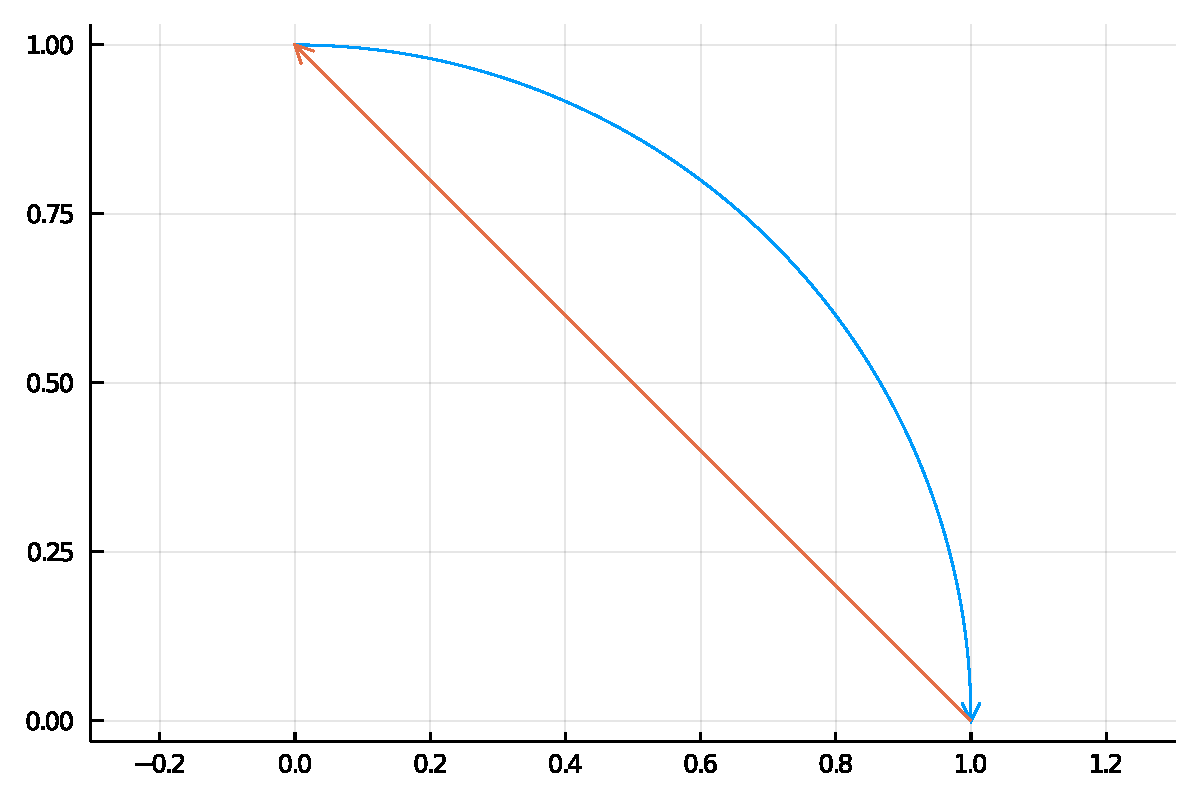
\includegraphics[width=0.95\linewidth]{C:/Users/mfaso/OneDrive/Documents/GitHub/M3M6AppliedComplexAnalysis/output/figures/Lecture2_14_1.pdf}}

The starting point of our review was the following construction:

\begin{itemize}
\item[1. ] Holomorphic functions


\item[2. ] Cauchy's theorem


\item[3. ] Deformation of contours


\item[4. ] Cauchy's integral formula


\item[5. ] Analyticity and Taylor series

\end{itemize}
We have discussed 1-3, that (1) integrating a holomorphic function over a simple closed contour returns zero and (2) therefore integrals over complex contours depend only on the start and end points provided the integrand is holomorphic in between. We now use these to review 4-5.

\newpage

\subsection{Cauchy's integral formula}
Contours are \emph{oriented}: there is a notion of "left" and "right" inherited from $[a,b]$. For closed contours, there is a notion of positive/negative orientation:

\textbf{Definition (Positive/negative orientation)} Let $\gamma$ be a simple closed contour and $z$ in the interior of $\gamma$.  We say that $\gamma$ is \emph{positively oriented} if ${1 \over 2 \pi i} \oint_\gamma {d\zeta \over \zeta - z} = 1$ It is \emph{negatively oriented} if the reversed contour $\gamma_{\rm reversed}(t) = \gamma(b+a-t)$ for $t \in [a,b]$ is positively oriented, or equivalently ${1 \over 2 \pi i} \oint_\gamma {d\zeta \over \zeta - z} = -1$

Cauchy's integral formula allows us to recover a function from knowledge of its values on a surrounding contour:
\newpage
\textbf{Theorem (Cauchy integral formula)} Suppose $f$ is holomorphic inside and on a positively oriented, simple, closed contour $\gamma$. Then

$$
f(z) = \begin{cases}
{1 \over 2 \pi \I} \oint_\gamma {f(\zeta) \over \zeta - z} \D \zeta & z \hbox{ inside $\gamma$} \\
0 & \hbox{ otherwise}
\end{cases}
$$

\textbf{Sketch of Proof}

Let $C_r := \{ z + r \E^{\I \theta} : 0 \leq \theta < 2\pi \}$ be a small circle around $z$ inside the domain of holomorphicity of $f$. Contour deformation informs us that

\[
\oint_\gamma {f(\zeta) \over \zeta - z} \D \zeta  =
\oint_{C_r} {f(\zeta) \over \zeta - z} \D \zeta =
\I \int_0^{2 \pi} f(z + r \E^{\I \theta})\D \theta =
2 \pi \I f(z) + \int_0^{2 \pi} {f(z + r \E^{\I \theta}) - f(z)} \D \theta.
\]
By continuity, the second integral tends to zero.

\ensuremath{\mdblksquare}

Not only do we know $f$, a consequence of this formula is  that $f$ is infinitely-differentiable by differentiating the integrand with respect to $z$, and we know all its values:

\textbf{Corollary (Cauchy integral formula for derivatives)} Suppose $f$ is holomorphic inside and on a positively oriented, simple, closed contour $\gamma$. Then $f$ is infinitely-differentiable at $z$ and

\[
f^{(k)}(z) = {k! \over 2 \pi i} \oint_\gamma {f(\zeta) \over (\zeta - z)^{k+1}} d \zeta
\]
\subsection{Taylor series}
\textbf{Theorem (Taylor)} Suppose $f$ is holomorphic in a ball $B(z_0,r)$. Then inside this ball we have

\[
    f(z) = {\displaystyle{\sum_{k=0}^\infty {f^{(k)}(z_0) \over k!} (z-z_0)^k}}
\]
\newpage
\textbf{Sketch of proof}

For simplicity, take $z_0 = 0$. This result follows from approximating the Cauchy kernel $1/(z - \zeta)$ by its geometric series. Recall by telescoping sum

\[
(1-z) (1 + z + \cdots + z^n) = 1 - z^{n+1}.
\]
Therefore

\[
{1 \over z - \zeta} = {1 \over -\zeta} {1 \over 1 - z/\zeta} = {1 \over - \zeta} (1 + (z/\zeta) + \cdots + (z/\zeta)^n + {(z/\zeta)^{n+1} \over 1 - z/\zeta})
\]
Thus for $C_r$, a circle of radius $r$, we have


\begin{align*}
f(z) &= {1 \over 2 \pi \I} \oint_{C_r} {f(\zeta) \over \zeta - z} \D \zeta \\
&=
\sum_{k=0}^n z^n {1 \over 2 \pi \I}  \oint_{C_r} f(\zeta) \zeta^{-n-1} \D \zeta + {1 \over 2 \pi \I} \oint_{C_r} f(\zeta)  {(z/\zeta)^{n+1} \over 1 - z/\zeta} \D \zeta \\
&=
\sum_{k=0}^n {f^{(k)}(0) \over k!} z^n + R_n(z)
\end{align*}
Because $|z| < r$ we have $|z/\zeta| < 1$ which implies the integrand in $R_n(z)$ uniformly tends to zero, i.e., $R_n(z) \rightarrow 0$ as $n \rightarrow \infty$.

\ensuremath{\mdblksquare}

\subsection{Demonstration}
Here we see numerically that $1/z$ is positively oriented:


\begin{lstlisting}
(*@\HLJLnf{sum}@*)(*@\HLJLp{(}@*)(*@\HLJLnf{Fun}@*)(*@\HLJLp{(}@*)(*@\HLJLn{z}@*) (*@\HLJLoB{->}@*) (*@\HLJLni{1}@*)(*@\HLJLoB{/}@*)(*@\HLJLn{z}@*)(*@\HLJLp{,}@*) (*@\HLJLnf{Circle}@*)(*@\HLJLp{()))}@*)(*@\HLJLoB{/}@*)(*@\HLJLp{(}@*)(*@\HLJLni{2}@*)(*@\HLJLn{\ensuremath{\pi}}@*)(*@\HLJLoB{*}@*)(*@\HLJLn{im}@*)(*@\HLJLp{)}@*)
\end{lstlisting}

\begin{lstlisting}
1.0 + 1.2545118101832475e-16im
\end{lstlisting}


This shows numerically that we can calculate $\E^{0.1}$ by integrating over a circle that surrounds $z = 0.1$:


\begin{lstlisting}
(*@\HLJLn{\ensuremath{\gamma}}@*) (*@\HLJLoB{=}@*) (*@\HLJLnf{Circle}@*)(*@\HLJLp{()}@*)
(*@\HLJLn{\ensuremath{\zeta}}@*) (*@\HLJLoB{=}@*) (*@\HLJLnf{Fun}@*)(*@\HLJLp{(}@*)(*@\HLJLn{\ensuremath{\gamma}}@*)(*@\HLJLp{)}@*)
(*@\HLJLn{z}@*) (*@\HLJLoB{=}@*) (*@\HLJLnfB{0.1}@*)
(*@\HLJLnf{sum}@*)(*@\HLJLp{(}@*)(*@\HLJLnf{exp}@*)(*@\HLJLp{(}@*)(*@\HLJLn{\ensuremath{\zeta}}@*)(*@\HLJLp{)}@*)(*@\HLJLoB{/}@*)(*@\HLJLp{(}@*)(*@\HLJLn{\ensuremath{\zeta}}@*)(*@\HLJLoB{-}@*)(*@\HLJLn{z}@*)(*@\HLJLp{))}@*) (*@\HLJLoB{/}@*)(*@\HLJLp{(}@*)(*@\HLJLni{2}@*)(*@\HLJLn{\ensuremath{\pi}}@*)(*@\HLJLoB{*}@*)(*@\HLJLn{im}@*)(*@\HLJLp{)}@*)  (*@\HLJLoB{-}@*) (*@\HLJLnf{exp}@*)(*@\HLJLp{(}@*)(*@\HLJLn{z}@*)(*@\HLJLp{)}@*)
\end{lstlisting}

\begin{lstlisting}
-4.440892098500626e-16 - 0.0im
\end{lstlisting}


Here we show that we can recover $\E^z$ using any of the derivatives:


\begin{lstlisting}
(*@\HLJLn{k}@*)(*@\HLJLoB{=}@*)(*@\HLJLni{10}@*)
(*@\HLJLnf{factorial}@*)(*@\HLJLp{(}@*)(*@\HLJLnfB{1.0}@*)(*@\HLJLn{k}@*)(*@\HLJLp{)}@*)(*@\HLJLoB{*}@*)(*@\HLJLnf{sum}@*)(*@\HLJLp{(}@*)(*@\HLJLnf{exp}@*)(*@\HLJLp{(}@*)(*@\HLJLn{\ensuremath{\zeta}}@*)(*@\HLJLp{)}@*)(*@\HLJLoB{/}@*)(*@\HLJLp{(}@*)(*@\HLJLn{\ensuremath{\zeta}}@*)(*@\HLJLoB{-}@*)(*@\HLJLn{z}@*)(*@\HLJLp{)}@*)(*@\HLJLoB{{\textasciicircum}}@*)(*@\HLJLp{(}@*)(*@\HLJLn{k}@*)(*@\HLJLoB{+}@*)(*@\HLJLni{1}@*)(*@\HLJLp{))}@*)(*@\HLJLoB{/}@*)(*@\HLJLp{(}@*)(*@\HLJLni{2}@*)(*@\HLJLn{\ensuremath{\pi}}@*)(*@\HLJLoB{*}@*)(*@\HLJLn{im}@*)(*@\HLJLp{)}@*)  (*@\HLJLoB{-}@*) (*@\HLJLnf{exp}@*)(*@\HLJLp{(}@*)(*@\HLJLn{z}@*)(*@\HLJLp{)}@*)
\end{lstlisting}

\begin{lstlisting}
2.294213707898507e-10 - 0.0im
\end{lstlisting}


\begin{lstlisting}
(*@\HLJLn{z}@*) (*@\HLJLoB{=}@*) (*@\HLJLnfB{0.1}@*)
(*@\HLJLn{k}@*) (*@\HLJLoB{=}@*) (*@\HLJLni{5}@*)
(*@\HLJLnf{factorial}@*)(*@\HLJLp{(}@*)(*@\HLJLnfB{1.0}@*)(*@\HLJLn{k}@*)(*@\HLJLp{)}@*)(*@\HLJLoB{*}@*)(*@\HLJLnf{sum}@*)(*@\HLJLp{(}@*)(*@\HLJLnf{exp}@*)(*@\HLJLp{(}@*)(*@\HLJLn{\ensuremath{\zeta}}@*)(*@\HLJLp{)}@*)(*@\HLJLoB{/}@*)(*@\HLJLp{(}@*)(*@\HLJLn{\ensuremath{\zeta}}@*)(*@\HLJLoB{-}@*)(*@\HLJLn{z}@*)(*@\HLJLp{)}@*)(*@\HLJLoB{{\textasciicircum}}@*)(*@\HLJLp{(}@*)(*@\HLJLn{k}@*)(*@\HLJLoB{+}@*)(*@\HLJLni{1}@*)(*@\HLJLp{))}@*)(*@\HLJLoB{/}@*)(*@\HLJLp{(}@*)(*@\HLJLni{2}@*)(*@\HLJLn{\ensuremath{\pi}}@*)(*@\HLJLoB{*}@*)(*@\HLJLn{im}@*)(*@\HLJLp{)}@*) (*@\HLJLoB{-}@*) (*@\HLJLnf{exp}@*)(*@\HLJLp{(}@*)(*@\HLJLn{z}@*)(*@\HLJLp{)}@*)
\end{lstlisting}

\begin{lstlisting}
2.1094237467877974e-14 - 0.0im
\end{lstlisting}


For Taylor series, we consider the following examples:

\begin{itemize}
\item[1. ] \[
\E^z
\]

\item[2. ] \[
1/(1-z)
\]

\item[3. ] \[
\sec z
\]

\item[4. ] \[
\sqrt z
\]
\end{itemize}
\newpage
Here we plot the $n$-term Taylor approximation of $\E^z$:


\begin{lstlisting}
(*@\HLJLn{exp{\_}n}@*) (*@\HLJLoB{=}@*) (*@\HLJLp{(}@*)(*@\HLJLn{n}@*)(*@\HLJLp{,}@*)(*@\HLJLn{z}@*)(*@\HLJLp{)}@*) (*@\HLJLoB{->}@*) (*@\HLJLnf{sum}@*)(*@\HLJLp{(}@*)(*@\HLJLn{z}@*)(*@\HLJLoB{{\textasciicircum}}@*)(*@\HLJLn{k}@*)(*@\HLJLoB{/}@*)(*@\HLJLnf{factorial}@*)(*@\HLJLp{(}@*)(*@\HLJLnfB{1.0}@*)(*@\HLJLn{k}@*)(*@\HLJLp{)}@*) (*@\HLJLk{for}@*) (*@\HLJLn{k}@*)(*@\HLJLoB{=}@*)(*@\HLJLni{0}@*)(*@\HLJLoB{:}@*)(*@\HLJLn{n}@*)(*@\HLJLp{)}@*)
(*@\HLJLnf{phaseplot}@*)(*@\HLJLp{(}@*)(*@\HLJLoB{-}@*)(*@\HLJLnfB{20..20}@*)(*@\HLJLp{,}@*) (*@\HLJLoB{-}@*)(*@\HLJLnfB{20..20}@*)(*@\HLJLp{,}@*) (*@\HLJLn{z}@*) (*@\HLJLoB{->}@*) (*@\HLJLn{exp{\_}n}@*)(*@\HLJLoB{.}@*)(*@\HLJLp{(}@*)(*@\HLJLni{10}@*)(*@\HLJLp{,}@*)(*@\HLJLn{z}@*)(*@\HLJLp{))}@*)
\end{lstlisting}

\cent{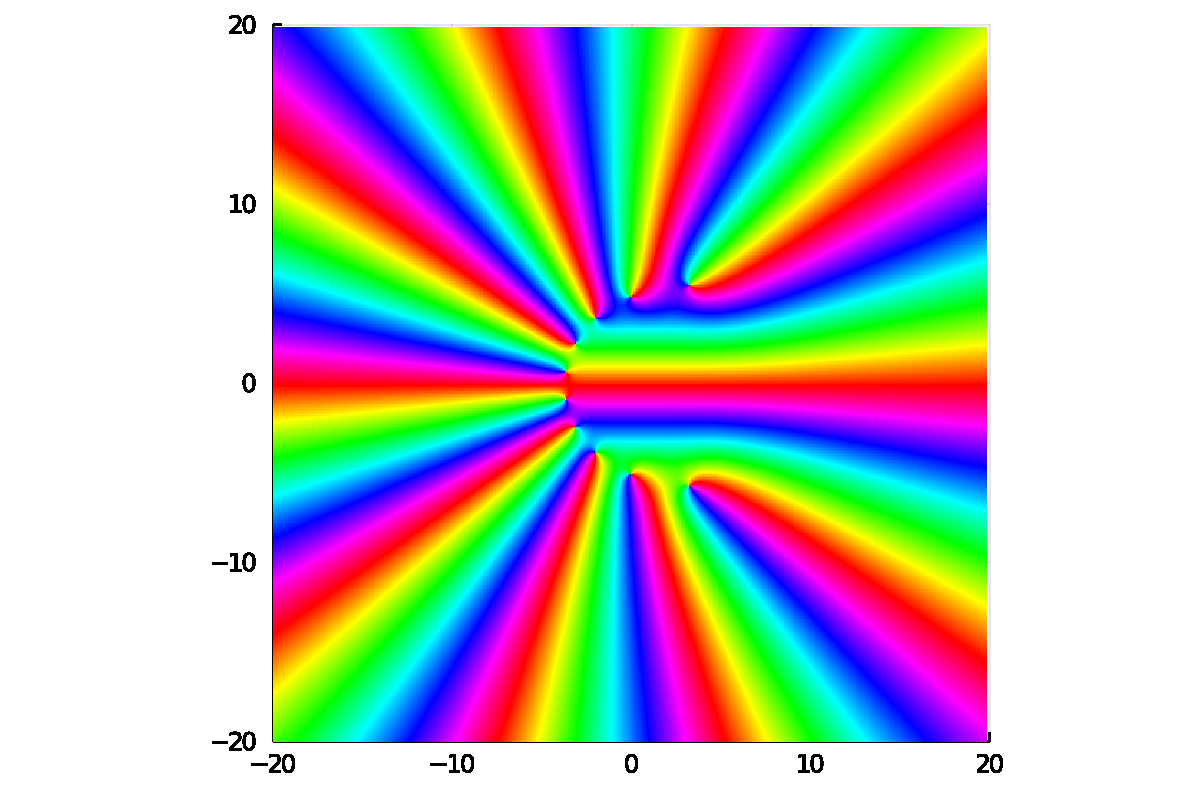
\includegraphics[width=0.85\linewidth]{C:/Users/mfaso/OneDrive/Documents/GitHub/M3M6AppliedComplexAnalysis/output/figures/Lecture2_19_1.pdf}}

This shows that we accurately approximate the function $\E^z$ inside a disk, and this disk grows with \texttt{n}.\newpage

And now the $n$-term Taylor approximation to $1/(1-z)$:


\begin{lstlisting}
(*@\HLJLn{geometric{\_}n}@*) (*@\HLJLoB{=}@*) (*@\HLJLp{(}@*)(*@\HLJLn{n}@*)(*@\HLJLp{,}@*)(*@\HLJLn{z}@*)(*@\HLJLp{)}@*) (*@\HLJLoB{->}@*) (*@\HLJLnf{sum}@*)(*@\HLJLp{(}@*)(*@\HLJLn{z}@*)(*@\HLJLoB{{\textasciicircum}}@*)(*@\HLJLn{k}@*) (*@\HLJLk{for}@*) (*@\HLJLn{k}@*)(*@\HLJLoB{=}@*)(*@\HLJLni{0}@*)(*@\HLJLoB{:}@*)(*@\HLJLn{n}@*)(*@\HLJLp{)}@*)

(*@\HLJLnf{phaseplot}@*)(*@\HLJLp{(}@*)(*@\HLJLoB{-}@*)(*@\HLJLnfB{2..2}@*)(*@\HLJLp{,}@*) (*@\HLJLoB{-}@*)(*@\HLJLnfB{2..2}@*)(*@\HLJLp{,}@*) (*@\HLJLn{z}@*) (*@\HLJLoB{->}@*) (*@\HLJLn{geometric{\_}n}@*)(*@\HLJLoB{.}@*)(*@\HLJLp{(}@*)(*@\HLJLni{20}@*)(*@\HLJLp{,}@*)(*@\HLJLn{z}@*)(*@\HLJLp{))}@*)
\end{lstlisting}

\cent{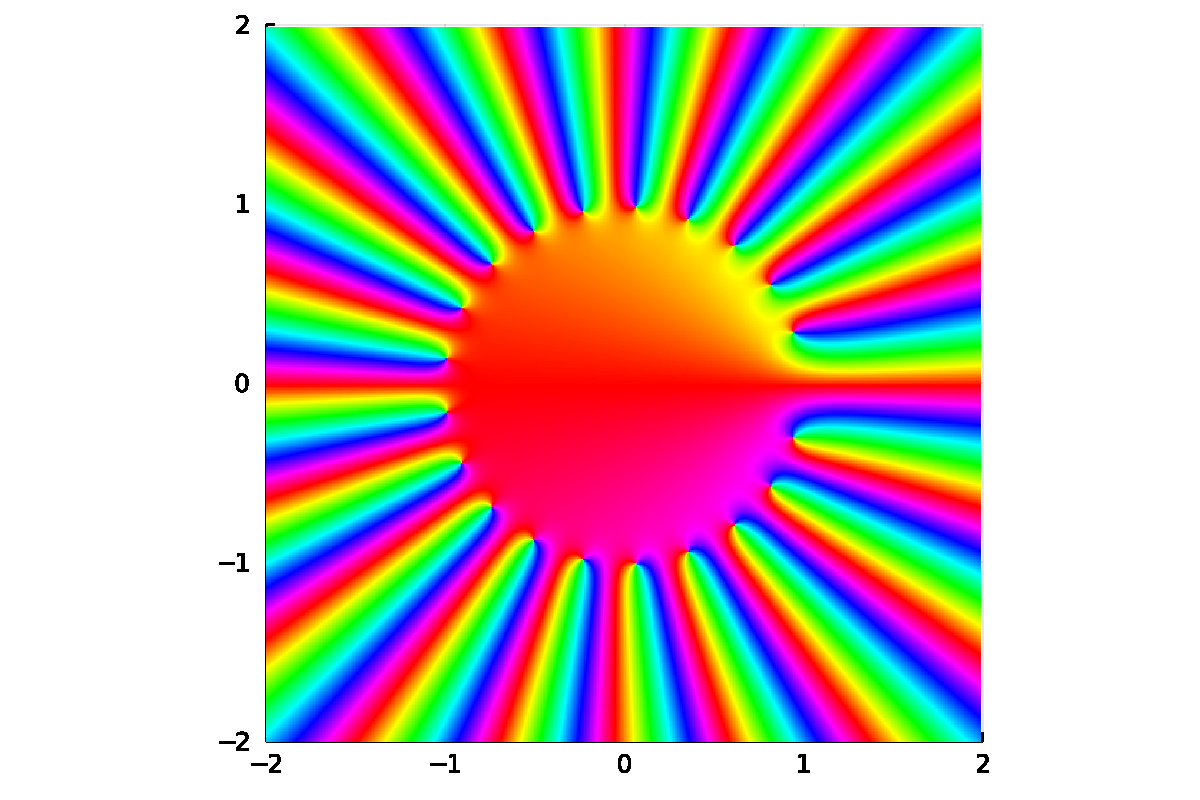
\includegraphics[width=0.9\linewidth]{C:/Users/mfaso/OneDrive/Documents/GitHub/M3M6AppliedComplexAnalysis/output/figures/Lecture2_20_1.pdf}}

And here the $n$-term Taylor approximation of $\sqrt z$ near $z_0$:


\begin{lstlisting}
(*@\HLJLk{function}@*) (*@\HLJLnf{sqrt{\_}n}@*)(*@\HLJLp{(}@*)(*@\HLJLn{n}@*)(*@\HLJLp{,}@*)(*@\HLJLn{z}@*)(*@\HLJLp{,}@*)(*@\HLJLn{z\ensuremath{\_0}}@*)(*@\HLJLp{)}@*)
    (*@\HLJLn{ret}@*) (*@\HLJLoB{=}@*) (*@\HLJLnf{sqrt}@*)(*@\HLJLp{(}@*)(*@\HLJLn{z\ensuremath{\_0}}@*)(*@\HLJLp{)}@*)
    (*@\HLJLn{c}@*) (*@\HLJLoB{=}@*) (*@\HLJLnfB{0.5}@*)(*@\HLJLoB{/}@*)(*@\HLJLn{ret}@*)(*@\HLJLoB{*}@*)(*@\HLJLp{(}@*)(*@\HLJLn{z}@*)(*@\HLJLoB{-}@*)(*@\HLJLn{z\ensuremath{\_0}}@*)(*@\HLJLp{)}@*)
    (*@\HLJLk{for}@*) (*@\HLJLn{k}@*)(*@\HLJLoB{=}@*)(*@\HLJLni{1}@*)(*@\HLJLoB{:}@*)(*@\HLJLn{n}@*)
        (*@\HLJLn{ret}@*) (*@\HLJLoB{+=}@*) (*@\HLJLn{c}@*)
        (*@\HLJLn{c}@*) (*@\HLJLoB{*=}@*) (*@\HLJLoB{-}@*)(*@\HLJLp{(}@*)(*@\HLJLni{2}@*)(*@\HLJLn{k}@*)(*@\HLJLoB{-}@*)(*@\HLJLni{1}@*)(*@\HLJLp{)}@*)(*@\HLJLoB{/}@*)(*@\HLJLp{(}@*)(*@\HLJLni{2}@*)(*@\HLJLoB{*}@*)(*@\HLJLp{(}@*)(*@\HLJLn{k}@*)(*@\HLJLoB{+}@*)(*@\HLJLni{1}@*)(*@\HLJLp{)}@*)(*@\HLJLoB{*}@*)(*@\HLJLn{z\ensuremath{\_0}}@*)(*@\HLJLp{)}@*)(*@\HLJLoB{*}@*)(*@\HLJLp{(}@*)(*@\HLJLn{z}@*)(*@\HLJLoB{-}@*)(*@\HLJLn{z\ensuremath{\_0}}@*)(*@\HLJLp{)}@*)
    (*@\HLJLk{end}@*)
    (*@\HLJLn{ret}@*)
(*@\HLJLk{end}@*)
\end{lstlisting}
\newpage
\begin{lstlisting}
(*@\HLJLn{z\ensuremath{\_0}}@*) (*@\HLJLoB{=}@*) (*@\HLJLnfB{0.3}@*)
(*@\HLJLn{n}@*) (*@\HLJLoB{=}@*) (*@\HLJLni{40}@*)
(*@\HLJLnf{phaseplot}@*)(*@\HLJLp{(}@*)(*@\HLJLoB{-}@*)(*@\HLJLnfB{2..2}@*)(*@\HLJLp{,}@*) (*@\HLJLoB{-}@*)(*@\HLJLnfB{2..2}@*)(*@\HLJLp{,}@*) (*@\HLJLn{z}@*) (*@\HLJLoB{->}@*) (*@\HLJLn{sqrt{\_}n}@*)(*@\HLJLoB{.}@*)(*@\HLJLp{(}@*)(*@\HLJLn{n}@*)(*@\HLJLp{,}@*)(*@\HLJLn{z}@*)(*@\HLJLp{,}@*)(*@\HLJLn{z\ensuremath{\_0}}@*)(*@\HLJLp{))}@*)
\end{lstlisting}

\cent{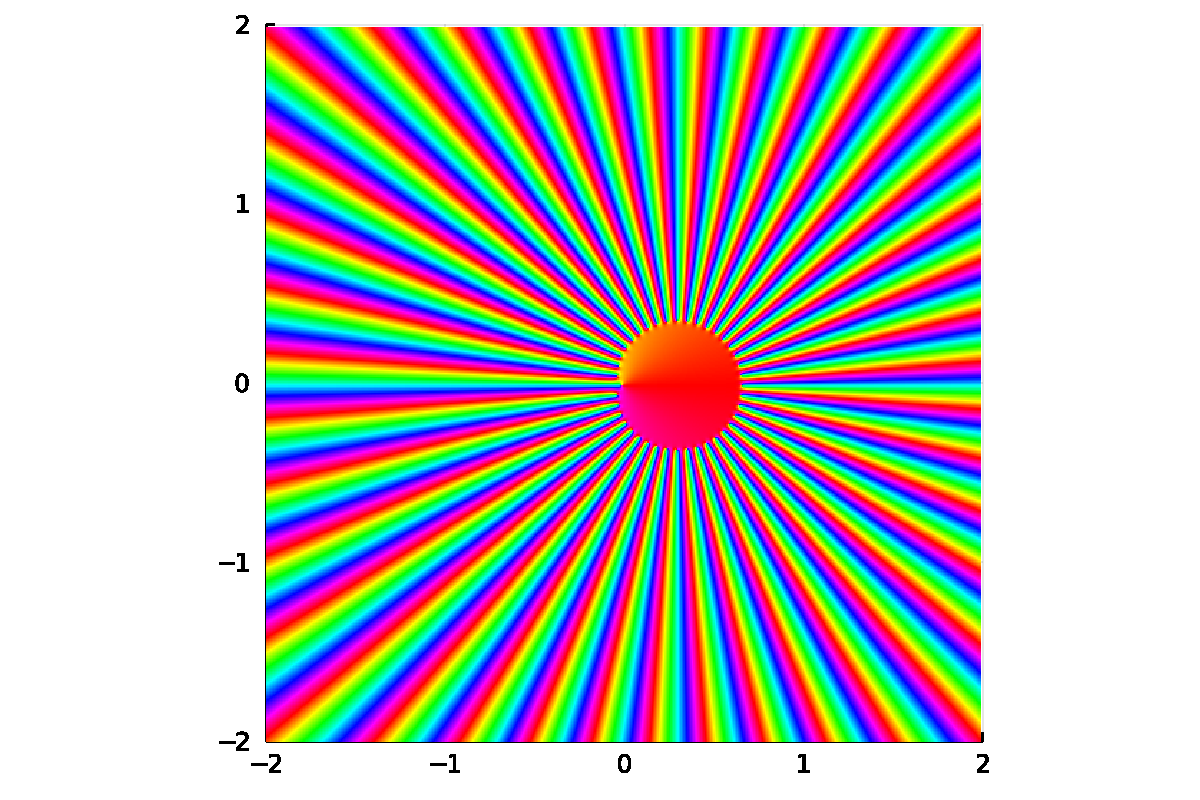
\includegraphics[width=0.95\linewidth]{C:/Users/mfaso/OneDrive/Documents/GitHub/M3M6AppliedComplexAnalysis/output/figures/Lecture2_21_1.pdf}}

}
\end{document}
